\section[CNNs]{Convolutional neural networks}

\subsection{}

\begin{frame}
    \frametitle{Motivation}

    \begin{block}{Disclaimer}
        I know almost nothing about CNNs, but not discussing them would be sacrilegious.
        I'll do my best.
    \end{block}
    \pause

    \begin{itemize}
        \item Much of deep learning revolves around image classification
        \item A huge proportion of early major breakthroughs in deep learning involved CNNs for image classification
    \end{itemize}
    \pause

    \begin{block}{Spatial invariance}
        CNNs leverage the fact that images are \alert{spatially invariant}
        \begin{itemize}
            \item A dog is a dog whether its head is in the left or right side of an image
            \item Dense networks treat every input as independent
        \end{itemize}
    \end{block}
\end{frame}

\begin{frame}
    \frametitle{2-D convolution}
    \begin{columns}
        \begin{column}{0.41\textwidth}
            \begin{tikzpicture}[x=1.5mm, y=1.5mm, auto]
    \foreach \depth in {2, ..., 0} {
        \visible<1-2>{\image{-\depth}{\depth}}
        \visible<2>{\filter{-\depth}{-28 + \depth}}
    }

    \visible<1>{
        \draw [Latex-Latex] (0, -21) -- node [below, font=\footnotesize] {$w$} (20, -21);
        \draw [Latex-Latex] (21, 0) -- node [font=\footnotesize] {$h$} (21, -20);
        \draw [Latex-Latex] (-1, -21) -- node [below, font=\footnotesize, rotate=315] {$3$} (-3, -19);
    }

    \visible<2>{
        \draw [Latex-Latex] (0, -34) -- node [below, font=\footnotesize] {$m$} (5, -34);
        \draw [Latex-Latex] (6, -28) -- node [font=\footnotesize] {$m$} (6, -33);
        \draw [Latex-Latex] (-1, -34) -- node [below, font=\footnotesize, rotate=315] {$3$} (-3, -32);
    }

    \foreach \i in {0, ..., 5} {
        \pgfmathtruncatemacro{\overlay}{\i + 3}
        \foreach \depth in {2, ..., 0} {
            \visible<\overlay>{
                \image{-\depth}{\depth}
                \filter{\i - \depth}{\depth}
            }
        }

        \visible<\overlay->{\featuremap{\i + 4}{-28}{1}}
        \visible<\overlay>{\draw [path] (\i + 2.5, -2.5) -- (\i + 4.5, -28.5);}
    }

    \visible<9>{
        \foreach \depth in {2, ..., 0} {
            \image{-\depth}{\depth}
            \filter{15 - \depth}{-15 + \depth}
        }

        \featuremap{4}{-28}{16}
        \draw [path] (17.5, -17.5) -- (19.5, -43.5);
    }

    \visible<9->{
        \draw [Latex-Latex] (4, -45) -- node [below, font=\footnotesize] {$w - m + 1$} (20, -45);
        \draw [Latex-Latex] (21, -28) -- node [below, font=\footnotesize, rotate=90] {$h - m + 1$} (21, -44);
    }

    \visible<10->{
        \foreach \depth in {2, ..., 0} {
            \image{-\depth}{\depth}
        }

        \foreach \depth in {5, ..., 0} {
            \featuremap{4 - \depth}{-28 + \depth}{16}
        }

        \draw [Latex-Latex] (3, -45) -- node [below, font=\footnotesize, rotate=315] {$k$} (-2, -40);
    }
\end{tikzpicture}
%%% Local Variables:
%%% mode: latex
%%% TeX-master: "../nn"
%%% End:

        \end{column}
        \begin{column}{0.59\textwidth}
            Given
            \begin{itemize}[<+->]
                \item \textcolor{blue}{RGB image}, dimension $w \times h \times 3$
                \item A \alert{filter}/\alert{kernel}, dimension $m \times m \times 3$, $m = \O(1 \text{--} 10) \ll w, h$
            \end{itemize}
            \uncover<+->{For every $m \times m$ block in the 2-D image:}
            \begin{itemize}[<.->]
                \item Element-wise multiply $m \times m \times 3$ block by filter ($\Reals^{m \times m \times 3} \to \Reals^{m \times m \times 3}$)
                \item Sum the result ($\Reals^{m \times m \times 3} \to \Reals$)
                \setcounter{beamerpauses}{9}
                \item<+-> $w - m + 1$ horizontal block positions \& $h - m + 1$ vertical block positions $\implies$ produces \textcolor{Green4}{feature map} in $\Reals^{(w-m+1) \times (h-m+1)}$
            \end{itemize}

            \uncover<+->{Repeat for $k$ filters}
            \begin{itemize}
                \item<.-> Yields $k$ feature maps in $\Reals^{(w-m+1) \times (h-m+1) \times k}$
            \end{itemize}

            \uncover<+->{Can take $\text{\alert{stride}} > 1$ when sliding filter}
        \end{column}
    \end{columns}
\end{frame}

\begin{frame}
    \frametitle{What's the point?}

    \begin{columns}
        \begin{column}{0.31\textwidth}
            \begin{tikzpicture}[x=1.5mm, y=1.5mm, auto]
    % The image.
    \foreach \depth in {2, ..., 0} {
        \image{-\depth}{\depth}
    }

    % Tires.
    \foreach \i in {5.5, 15.5} {
        \draw [very thick] (\i, -9.5) circle (1.5);
    }

    % Complete the feature map.
    \featuremap{4}{-28}{16}

    \foreach \i in {5.5, 15.5} {
        \filter{\i - 2.5}{-7} % A filter matching the tire.
        \draw [very thick] (\i, -9.5) circle (1.5); % Tires.

        % Lit-up feature map elements.
        \draw [very thick, fill=green] (\i + 1.5, -35) rectangle (\i + 2.5, -36);
        \draw [path] (\i, -9.5) -- (\i + 2, -35.5);
    }
\end{tikzpicture}
%%% Local Variables:
%%% mode: latex
%%% TeX-master: "../nn"
%%% End:

        \end{column}
        \begin{column}{0.69\textwidth}
            Overly simplified example:
            \begin{itemize}[<+->]
                \item Suppose one of the class label is ``car''
                \item Cars have wheels
                \item Suppose one of the filters has a round shape
                \item For most $m \times m \times 3$ blocks, convolution produces noise
                \setcounter{beamerpauses}{10}
                \item If block contains tire, then convolution hits $\implies$ large value
            \end{itemize}

            \uncover<+->{The abstract idea: CNNs surpass dense NNs for images because}
            \begin{itemize}[<.->]
                \item \alert{Sparse connectivity}: $(\text{filter size}) \ll (\text{image size})$
                \item \alert{Shared parameters}/\alert{tied weights}: same filters applied to every block in image
            \end{itemize}
        \end{column}
    \end{columns}
\end{frame}

\begin{frame}
    \frametitle{Filters, pooling, \& downsampling}

    \begin{columns}
        \begin{column}{0.4\textwidth}
            \centering
            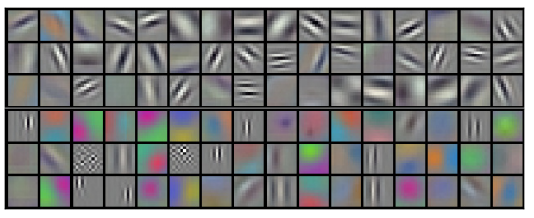
\includegraphics[width=\textwidth]{filters} \\
            {\footnotesize AlexNet filters \citep{KrizhevskyNIPS12}}
            \vspace{5mm}

            \begin{tikzpicture}[
    x=4mm,
    y=4mm,
    number/.style={
        draw,
        rectangle,
        minimum width=4mm,
        minimum height=4mm,
        fill=green!20,
        font=\small,
        inner sep=1pt
    }
]
    \setcounter{beamerpauses}{2}

    % The detector stage outputs.
    \visible<+->{
        \foreach \i/\n in {0/9, 1/0, 2/3, 3/5, 4/0} {
            \node (conv 0\i) at (\i, 0) [number] {\n};
        }

        \foreach \i/\n in {0/8, 1/4, 2/4, 3/1, 4/7} {
            \node (conv 1\i) at (\i, -1) [number] {\n};
        }

        \foreach \i/\n in {0/4, 1/1, 2/2, 3/4, 4/5} {
            \node (conv 2\i) at (\i, -2) [number] {\n};
        }

        \foreach \i/\n in {0/2, 1/3, 2/3, 3/4, 4/3} {
            \node (conv 3\i) at (\i, -3) [number] {\n};
        }

        \foreach \i/\n in {0/3, 1/9, 2/6, 3/2, 4/1} {
            \node (conv 4\i) at (\i, -4) [number] {\n};
        }
    }

    % Start pooling, one by one.
    \visible<+->{\node (pool 00) at (0, -6) [number] {9};}
    \visible<.>{
        \draw [very thick] (-0.5, 0.5) rectangle (1.5, -1.5);
        \draw [path] (conv 10.315) -- (pool 00);
    }

    \foreach \i\n in {1/9, 2/5, 3/7} {
        \visible<+->{\node (pool 0\i) at (\i, -6) [number] {\n};}

        \visible<.>{
            \draw [very thick] (\i - 1.5, 0.5) rectangle (\i + 1.5, -1.5);
            \draw [path] (conv 1\i) -- (pool 0\i);
        }
    }

    \visible<+->{\node (pool 04) at (4, -6) [number] {7};}
    \visible<.>{
        \draw [very thick] (2.5, 0.5) rectangle (4.5, -1.5);
        \draw [path] (conv 14.225) -- (pool 04);
    }

    \visible<+->{\node (pool 10) at (0, -7) [number] {9};}
    \visible<.>{
        \draw [very thick] (-0.5, 0.5) rectangle (1.5, -2.5);
        \draw [path] (conv 20.315) -- (pool 10);
    }

    \foreach \i\n in {1/9, 2/5} {
        \visible<+->{\node (pool 1\i) at (\i, -7) [number] {\n};}

        \visible<.>{
            \draw [very thick] (\i - 1.5, 0.5) rectangle (\i + 1.5, -2.5);
            \draw [path] (conv 2\i) -- (pool 1\i);
        }
    }

    % The rest of the pooling.
    \visible<+->{
        \foreach \i/\n in {3/7, 4/7} {
            \node at (\i, -7) [number] {\n};
        }
        \foreach \i/\n in {0/8, 1/8, 2/4, 3/7, 4/7} {
            \node (pool 2\i) at (\i, -8) [number] {\n};
        }
        \foreach \i/\n in {0/9, 1/9, 2/9, 3/6, 4/5} {
            \node at (\i, -9) [number] {\n};
        }
        \foreach \i/\n in {0/9, 1/9, 2/9, 3/6, 4/4} {
            \node at (\i, -10) [number] {\n};
        }
    }

    % Downsampling.
    \visible<+->{
        \foreach \i in {0, 2} {
            \foreach \j in {0, -2} {
                \draw [very thick] (\i + 0.5, \j - 6.5) rectangle (\i + 1.5, \j - 7.5);
            }
        }

        \draw [-Latex, ultra thick] (pool 24) -- (6.5, -8);
    }

    \visible<.->{
        \node at (7, -7.5) [number] {9};
        \node at (8, -7.5) [number] {7};
        \node at (7, -8.5) [number] {9};
        \node at (8, -8.5) [number] {6};
    }
\end{tikzpicture}
%%% Local Variables:
%%% mode: latex
%%% TeX-master: "../nn"
%%% End:

        \end{column}

        \begin{column}{0.6\textwidth}
            Reality not that simple
            \begin{itemize}
                \item Trained filters find edges, arcs, color patches, etc.
            \end{itemize}

            \setcounter{beamerpauses}{2}
            \uncover<+->{Next, add bias and apply nonlinear activation function, then\ldots}

            \begin{block}{Pooling}<+->
                Replace each output with some statistic (e.g., max) on nearby region
            \end{block}

            \begin{itemize}[<.->]
                \item Improves invariance: makes exact positions less important
            \end{itemize}

            \begin{block}{Downsampling}<12->
                Reduces dimensionality for efficiency
            \end{block}
        \end{column}
    \end{columns}
\end{frame}

\begin{frame}
    \frametitle{Adding depth}

    \begin{tikzpicture}[x=1.5mm, y=1.5mm, auto]
    \foreach \depth in {5, ..., 0} {
        \featuremap{4 - \depth}{\depth}{16}
    }
\end{tikzpicture}

%%% Local Variables:
%%% mode: latex
%%% TeX-master: "../nn"
%%% End:


    So we have feature maps that light up when patterns match.
    Now what?%
\end{frame}

\begin{frame}
    \frametitle{Rich history that authors expect you to know}
    \begin{columns}
        \begin{column}{0.55\textwidth}
            \begin{itemize}
                \item<+-> Late 1990s: MNIST database of handwritten digits
                \begin{itemize}
                    \item 60,000 training samples, 10,000 test samples
                    \item $28 \times 28$ pixels, black and white
                    \item CNN test error: 0.7\% \citep[``LeNet-5'',][]{LeCunIEEE98} to 0.21\% \citep{WanICML13}
                \end{itemize}
                \item<+-> Early 2010s: CIFAR-10/100 database, 10/100 image labels
                \begin{itemize}
                    \item 50,000 training samples, 10,000 test samples
                    \item $32 \times 32$ color images
                    \item CIFAR-10 test error: 35\% \citep{RanzatoAISTATS10} to 2.1\% \citep{Real18}
                \end{itemize}
                \item<+-> Early 2010s: ImageNet---$\O(10^7)$ images, $\O(10^4)$ labels
            \end{itemize}
        \end{column}
        \begin{column}{0.45\textwidth}
            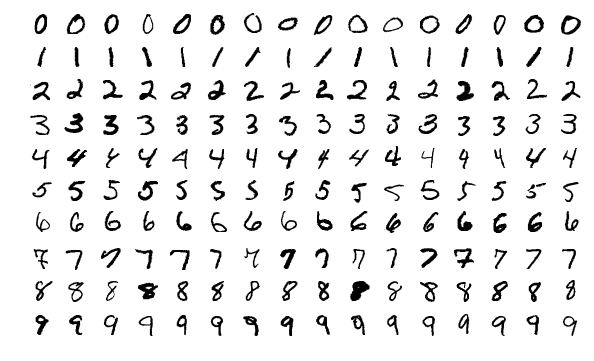
\includegraphics[width=\textwidth]{mnist} \\[5mm]
            \uncover<.->{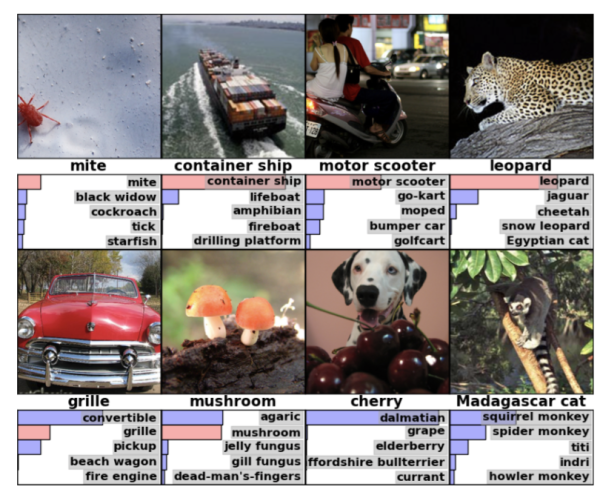
\includegraphics[width=\textwidth]{imagenet}}
        \end{column}
    \end{columns}
\end{frame}

\begin{frame}
    \frametitle{CNN architectures that authors expect you to know}

    \% ImageNet test samples with labels not in top 5:
    \begin{itemize}
        \item<+-> LeNet \citep{LeCunIEEE98}: 18.9\% top-5 error
        \begin{itemize}
            \item 2 convolutional layers (size $5 \times 5 \times 6$, $5 \times 5 \times 6 \times 16$) $\to$ 3 dense layers (size 120, 84, 10)
        \end{itemize}
        \item<+-> AlexNet \citep{KrizhevskyNIPS12}: 17.0\%
        \begin{itemize}
            \item 5 convolutional layers (size $11 \times 11 \times 3 \times 96$, $5 \times 5 \times 48 \times 256$, $3 \times 3 \times 256 \times 384$, $3 \times 3 \times 192 \times 384$, $3 \times 3 \times 192 \times 256$) $\to$ 3 dense layers (size 4096, 4096, 1000)
        \end{itemize}
        \item<+-> ZF Net \citep{ZeilerECCV14}: 11.2\%
        \begin{itemize}
            \item Minor improvement to AlexNet
        \end{itemize}
        \item<+-> VGGNet \citep{Simonyan14}: 7.7\%
        \begin{itemize}
            \item Replace AlexNet's $11 \times 11$ and $5 \times 5$ filters with deep $3 \times 3$ filters
        \end{itemize}
        \item<+-> GoogLeNet/Inception \citep{SzegedyIEEECVPR15}: 6.67\%
        \begin{itemize}
            \item Reduces work by using \emph{Inception modules} that combine size 1, 3, and 5 convolutions
        \end{itemize}
        \item<+-> ResNet \citep{He15b}: 3.57\%
        \begin{itemize}
            \item Instead of feeding convolutional output to next layer, feed convolutional input + output
        \end{itemize}
    \end{itemize}
\end{frame}

%%% Local Variables:
%%% mode: latex
%%% TeX-master: "../nn"
%%% End:
